
\chapter{Сплинты корневых систем и функции ветвления}
\label{cha:splints}


\section{Сплинты и ветвления}
\label{sec:splints}


%%\newtheorem{Def}{Definition}[section]
%%\newtheorem{Cnj}[Def]{Conjecture}
%%\newtheorem{Prop}[Def]{Property}
%%\newtheorem{example}{Example}[section]
%%
%\input{tcilatex}

Сплинт корневой системы простой алгебры Ли возникает при изучении регулярных вложений редуктивных подалгебр. Сплинт можно использовать для получения правил ветвления. Мы показываем, что использование свойств сплинта  позволяет сильно упростить вычисление коэффициентов ветвления. 

\section{Введение}
\label{sec:Introduction}

Вложение  $\phi$ корневой системы $\Delta_1$ в корневую систему $\Delta$ -- это биективное отображение корней из $\Delta_{1}$ в (собственное) подмножество $\Delta$, коммутирующее с законом сложения векторов в $\Delta_{1}$ и $\Delta$.

\begin{equation*}
\phi:\Delta_1 \longrightarrow \Delta
\end{equation*}
\begin{equation*}
\phi \circ (\alpha + \beta) =\phi \circ \alpha + \phi \circ \beta,
\,\,\, \alpha,\beta \in \Delta_1
\end{equation*}

Заметим, что образ  $Im(\phi)$ не обязан обладать свойствами корневой системы за исключением правил сложения, эквивалентных правилам сложения в  $\Delta_{1}$ (для прообразов). Два вложения  $\phi_1$ и $\phi_2$  {\it расщепляют} корневую систему  $\Delta$ если она может быть представлена, как несвязное объединение образов $Im(\phi_1)$ и $Im(\phi_2)$.   
Термин {\it сплинт} (расщепление) предложил D. Richter в работе  \cite{richter2008splints}, где  были получены все сплинты для простых алгебр Ли. В работе так же упоминалось, что сплинт должен быть тесно связан с конструкцией веера вложения. Веер вложения  $\Gamma\subset \Delta$ был введен в работе  \cite{lyakhovsky1996rra} как подмножество корневой системы, описывающее рекуррентные свойства коэффициентов ветвления для максимальных вложений. Веер вложения -- это эффективный инструмент для изучения правил ветвления. Позднее в работах \cite{2010arXiv1007.0318L, ilyin812pbc} эта конструкция была обобщена на не-максимальные вложения и бесконечномерные алгебры Ли.

В данной главе мы изучаем связь между сплинтом и веером вложения для регулярных вложений редуктивных подалгебр ${\mathfrak a}$ в простую алгебру Ли $\gf$. Мы демонстрируем, что (при выполнении определенных условий, описанных в разделе \ref{sec:stems and multiplicity functions}) сплинт является естественным инструментом для изучения свойств редукции  $\gf$-модулей по отношению к подалгебре $\af\longrightarrow\gf$. Используя этот инструмент мы получаем основной результат данной главы -- однозначное соответствие между кратностями весов неприводимых модулей сплинта и коэффициентов ветвления для редуцированного модуля $L^{\mu}_{\gf\downarrow \af}$

\section{Вложения и сплинты}

\label{sec:Injections and splints}

Рассмотрим простую алгебру Ли $\gf$ и ее  регулярную подалгебру $\af \hookrightarrow \gf$, такую, что $\af$ -- редуктивную подалгебра $\af\subset \gf$ и корневые системы согласованы $\hf_{\af}^{\ast}\subset\hf_{\gf}^{\ast}$. Пусть $\af^{\mathfrak{s}}$ -- полупростое слагаемое в $\mathfrak{a}$, то есть  $\af=\af^{\mathfrak{s}} \oplus \uf(1)\oplus \uf(1)\oplus \dots$. Мы будем считать, что $\af^{\mathfrak{s}}$ -- собственная регулярная подалгебра и что $\af$ -- максимальная подалгебра с заданной  $\af^{\mathfrak{s}}$, то есть ранг $r$ подалгебры $\af$ равен рангу $\gf$.


Пусть $L^{\mu }$ -- вполне приводимый по отношению к  $\af$ модуль алгебры $\gf$,
\[
L_{\gf\downarrow \af}^{\mu }=\bigoplus\limits_{\nu \in P_{\af%
}^{+}}b_{\nu }^{\left( \mu \right) }L_{\af}^{\nu }.
\]
\begin{equation}
\pi _{\af}ch\left( L^{\mu }\right) =\sum_{\nu \in P_{\af%
}^{+}}b_{\nu }^{(\mu )}ch\left( L_{\af}^{\nu }\right) .
\label{branching1}
\end{equation}
Для модулей, которые мы исследуем, формула Вейля для характеров $\mathrm{ch}\left(L^{\mu }\right) $ может быть записана через сингулярные элементы \cite{humphreys1997introduction}
\[
\Psi ^{\left( \mu \right) }:=\sum\limits_{w\in W}\epsilon (w)e^{w(\mu +\rho
)-\rho },
\]
а именно,
\begin{equation}
\mathrm{ch}\left( L^{\mu }\right) =\frac{\Psi ^{\left( \mu \right) }}{\Psi
^{\left( 0\right) }}=\frac{\Psi ^{\left( \mu \right) }}{R}.
\label{Weyl-Kac2}
\end{equation}
Это же верно и для подмодулей $\mathrm{ch}\left( L_{\af}^{\nu}\right) $ в уравнении (\ref{branching1})
\[
\mathrm{ch}\left( L_{\af}^{\nu }\right) =\frac{\Psi _{\af}^{\left(
\nu \right) }}{\Psi _{\af}^{\left( 0\right) }}=\frac{\Psi _{\af%
}^{\left( \nu \right) }}{R_{\af}},
\]
где
\[
\Psi _{\af}^{\left( \nu \right) }:=\sum\limits_{w\in W_{\af%
}}\epsilon (w)e^{w(\nu +\rho _{_{\af}})-\rho _{_{\af}}}.
\]

Применяя формулу (\ref{Weyl-Kac2}) к правилам ветвления (\ref{branching1}) мы получаем соотношение, связывающее сингулярные элементы $\Psi ^{\left( \mu\right) }$ и $\Psi _{\af}^{\left( \nu \right) }$ :
\begin{eqnarray}
\frac{\sum_{w \in W}\epsilon (w )e^{w (\mu +\rho )-\rho }}{\prod_{\alpha \in
\Delta ^{+}}(1-e^{-\alpha })} &=&\sum_{\nu \in P_{\af}^{+}}b_{\nu
}^{(\mu )}\frac{\sum_{w \in W_{\af}}\epsilon (w )e^{w (\nu +\rho _{%
\af})-\rho _{\af}}}{\prod_{\beta \in \Delta _{\af%
}^{+}}(1-e^{-\beta })},  \nonumber  \label{eq:4} \\
\frac{\Psi ^{\left( \mu \right) }}{R} &=&\sum_{\nu \in P_{\af%
}^{+}}b_{\nu }^{(\mu )}\frac{\Psi _{\af}^{\left( \nu \right) }}{R_{%
\af}}.  \label{singular main}
\end{eqnarray}

В работе \cite{2010arXiv1007.0318L} (см. главу \ref{cha:affine-lie-algebras}) было доказано, что коэффициенты ветвления $b_{\xi }^{\left(\mu\right)}$, отвечающие вложению $\af\hookrightarrow \gf$, удовлетворяют следующим рекуррентным соотношениям:
\begin{equation}
\begin{array}{c}
b_{\xi }^{\left( \mu \right) }=-\frac{1}{s\left( \gamma _{0}\right) }\left(
\sum_{u\in W/W_{\perp}}\epsilon (u)\;\dim \left( L_{\af_{\perp }}^{\mu _{\af%
_{\perp }}\left( u\right) }\right) \delta _{\xi -\gamma _{0},\pi _{%
\widetilde{\af}}(u(\mu +\rho )-\rho )}+\right. \\
\left. +\sum_{\gamma \in \Gamma _{\widetilde{\af}\rightarrow \gf%
}}s\left( \gamma +\gamma _{0}\right) b_{\xi +\gamma }^{\left( \mu \right)
}\right) ,
\end{array}
\label{recurrent rel}
\end{equation}
где $\afb$ -- подалгбера, задающаяся корнями  $\gf$, ортогональными ко всем корням $\af$ и $W_{\perp}$ -- подгруппа Вейля, соответствующая $\afb$,
\begin{eqnarray}
\Delta _{\af_{\perp }} &:&=\left\{ \beta \in \Delta _{\gf}|\forall
h\in \frak{h}_{\af};\beta \left( h\right) =0\right\} ,
\label{delta a ort}
\end{eqnarray}
\begin{eqnarray}
\widetilde{\af_{\perp }} :=\af_{\perp }\oplus \frak{h}_{\perp }
\qquad \widetilde{\af} :=\af\oplus \frak{h}_{\perp }
\end{eqnarray}
и $\pi$ -- оператор проекции. Если вложение максимально, то оператор проекции становится тривиальным и соотношение (\ref{recurrent rel}) упрощается:
\begin{equation}
\begin{array}{c}
b_{\xi }^{\left( \mu \right) }=-\frac{1}{s\left( \gamma _{0}\right) }\left(
\sum_{u\in W}\epsilon (u) \delta _{\xi -\gamma _{0}, u(\mu +\rho )-\rho
}+\right. \\
\left. +\sum_{\gamma \in \Gamma _{\af\rightarrow \gf}}s\left(
\gamma +\gamma _{0}\right) b_{\xi +\gamma }^{\left( \mu \right) }\right) .
\end{array}
\label{recurrent relation max}
\end{equation}
Рекурсия задается множеством  $\Gamma _{\af\rightarrow \gf}$, называющимся ``веер вложения''. Оно определяется как носитель $\left\{ \xi \right\} _{\af\rightarrow \gf}$ для коэффициентоной функции $s(\xi )$
\[
\left\{ \xi \right\} _{\af\rightarrow \gf}:=\left\{ \xi \in P_{%
\af}|s(\xi )\neq 0\right\}
\]
возникающей в разложении
\begin{equation}
\prod_{\alpha \in \Delta ^{+}\setminus \Delta _{\af}^{+}}\left( 1-e^{
-\alpha }\right) =-\sum_{\gamma \in P_{\af}}s(\gamma )e^{-\gamma };\quad
\label{product}
\end{equation}

Теперь мы приведем два определения, введенные в работе \cite{richter2008splints}

\begin{Def}
Пусть $\Delta _{0}$ и $\Delta$ -- корневые системы с соответствующими весовыми решетками $P_{0}$ и $P$. Тогда отображение $\phi $ -- ``вложение''
\begin{equation}
\phi :\left\{
\begin{array}{l}
\Delta _{0}\hookrightarrow \Delta , \\
P_{0}\hookrightarrow P,
\end{array}
\right.
\end{equation}
если \newline
\noindent (a) оно вкладывает $\Delta _{0}$ в $\Delta $, и \newline
\noindent (b) $\phi$ действует гомоморфно по отношению к группам сложения векторов в $P_{0}$ и $P$:
\[
\phi (\gamma )=\phi (\alpha )+\phi (\beta )
\]
для любой тройки $\alpha ,\beta ,\gamma \in P_{0}$, такой, что $\gamma =\alpha+\beta $.
\end{Def}

$\phi$ индуцирует вложение формальных алгебр: ${\mathcal{E}}_0\hookrightarrow \mathcal{E}$ и для образа ${\mathcal{E}}_i=\mathrm{Im}_{\phi}\left( {\mathcal{E}}_0\right)$ можно рассмотреть обратное отображение $\phi^{-1}:{\mathcal{E}}_i \longrightarrow {\mathcal{E}}_0$.

Заметим, что нужно различать два класса вложений: когда скалярное произведение (заданное формой Киллинга) в корневом пространстве $P_0$ инвариантно по отношению к  $\phi$ и когда оно не  $\phi$-инвариантно. Вложения первого класса называются ``метрическими'', второго -- ``неметрическими''. 

\begin{Def}
Корневая система $\Delta$ ``расщепляется'' на  $(\Delta _{1},\Delta _{2})$, если существует два вложения  $\phi _{1}:\Delta _{1}\hookrightarrow \Delta $ и $\phi _{2}:\Delta _{2}\hookrightarrow \Delta $, где (a) $\Delta $ -- несвязное объединение образов $\phi _{1}$ и $\phi _{2}$, и (b) ни ранг  $\Delta _{1}$, ни ранг  $\Delta _{2}$ не превосходит ранга $\Delta $.
\end{Def}

Эквивалентно, можно сказать, что  $(\Delta_1,\Delta_2)$  -- ``сплинт'' (расщепление)  $\Delta$ и мы можем обозначить его через $\Delta \approx (\Delta_1,\Delta_2)$. Каждая из компонент  $\Delta_1$ и $\Delta_2$ называется ``стеблем'' сплинта $(\Delta_1,\Delta_2)$.

Чтобы показать связь веера вложения со сплинтом рассмотрим случай, когда один из стеблей $\Delta _{1}=\Delta _{\af}$  является подсистемой корневой системы. 

Сплинт $\Delta \approx (\Delta _{1},\Delta _{2})$ называется ``инъективным'', если $\Delta _{1}=\Delta _{\af}$, -- подсистема корневой системы $\Delta $, соответствующая регулярной редуктивной подалгебре $\af\hookrightarrow \gf$. 

В случае инъективного сплинта второй стебель $\Delta _{\sfr}:=\Delta_{2}=\Delta \setminus \Delta _{\af}$ может быть переписан как произведение (\ref{product}) и определяет веер вложения  $\Gamma _{\af\hookrightarrow \gf}$. Обозначим через $\Delta_{\mathfrak{s}0}$ кообраз второго вложения $\phi:\Delta_{\mathfrak{s}0}\to \Delta_{\gf}$. Верна следующая гипотеза.

\begin{Cnj}
Каждый инъективный сплинт $\Delta \approx (\Delta _{\af},\Delta _{\sfr})$ определяет веер вложения с носителем $\left\{ \xi \right\} _{\af\rightarrow \gf}$, задающимся произведением
\begin{equation}
\prod_{\beta \in \Delta _{\sfr}^{+}}\left( 1-e^{-\beta }\right)
=-\sum_{\gamma \in P}s(\gamma )e^{-\gamma }\quad   \label{splint product}
\end{equation}
\end{Cnj}

В случае инъективного сплинты мы можем сказать, что подалгебра $\af\hookrightarrow \gf$ расщепляется $\Delta$ (и назовем $\af$ ``расщепляющей подалгеброй'' алгебры $\gf$).  Сплинты были классифицированы в работе \cite{richter2008splints}  (см. Приложение в работе) и первые три класса сплинтов в этой классификации инъективны. 

\section{Как стебли определяют функции кратности}

\label{sec:stems and multiplicity functions}

В этом разделе мы рассмотрим свойства инъективных сплинтов $\Delta \approx (\Delta _{\af},\Delta _{\sfr})$. Мы покажем, что в этом случае вычисление коэффициентов ветвления для расщепляющего вложения $\af\hookrightarrow\gf$ эквивалентно нахождению кратностей весов неприводимого $\sfr$-модуля $L_{\sfr}^{\nu }$ с определенным старшим весом $\nu $. Заметим, что алгебра $\sfr$ не обязательно должна быть подалгеброй $\gf$.

Вернемся к соотношению  (\ref{singular main}) и домножим обе стороны на  $R_{\af}$:
\begin{equation}
\frac{1}{\prod_{\beta \in \Delta _{\sfr}^{+}}(1-e^{-\beta })}\Psi _{\gf}^{\left( \mu \right) }=\sum_{\nu \in P_{\af}^{+}}b_{\nu}^{(\mu )}\Psi _{\af}^{\left( \nu \right) }.
\label{singular main-2}
\end{equation}
Здесь первый множитель в левой части -- это формальный элемент, обратный к вееру $\Gamma _{\af\rightarrow \gf}$. Рассмотрим модуль старшего веса $L_{\sfr}^{\nu }$. Вложение $\phi :\Delta _{\sfr\,0}\longrightarrow \Delta_{\gf}$ переводит сингулярный элемент  $\Psi _{\sfr}^{\left( \nu\right) }$ в $\Psi _{\gf}^{\left( \mu \right) }$. Применяя обратный морфизм $\phi ^{-1}$ к произведению $\left( \prod_{\beta \in \Delta_{\sfr}^{+}}(1-e^{-\beta })\right) ^{-1}\phi \left( \Psi _{\sfr}^{\left( \nu \right) }\right) $, мы получаем характер модуля $L_{\sfr}^{\nu }$,

\begin{equation}
\phi ^{-1}\left( \frac{1}{\prod_{\beta \in \Delta _{\sfr%
}^{+}}(1-e^{-\beta })}\phi \left( \Psi _{\sfr}^{\left( \nu \right)
}\right) \right) =\frac{1}{\prod_{\beta \in \Delta _{\sfr0
}^{+}}(1-e^{-\beta })}\Psi _{\sfr}^{\left( \nu \right) }=\mathrm{ch}%
\left( L_{\sfr}^{\nu }\right) .  \label{inverse for stem}
\end{equation}
Наша задача состоит в том, чтобы доказать, что сингулярный элемент $\Psi _{\gf}^{\left(\mu\right) }$ содержит элемент $\Psi _{\sfr}^{\left( \xi \right) }$ для модуля $L_{\sfr}^{\xi }$, однозначно определяемого модулем $L_{\gf}^{\mu }$ и что коэффициенты ветвления $b_{\nu }^{(\mu )}$ в правой части равенства (\ref{singular main-2}) совпадают с кратностями $m_{\zeta }^{\left( \xi\right) }$ соответствующих весов в $\mathcal{N}_{\sfr}^{\xi }$ .

Для неприводимого модуля старшего веса $L_{\gf}^{\mu }$ сингулярный элемент $\Psi _{\gf}^{\left( \mu \right) }$ -- это элемент $\mathcal{E}$, соответствующий сдвинутой орбите группы веса $\left( \mu +\rho\right) \in P^{+}$, со знаковой функцией $\epsilon \left( w\right) $. Удобно использовать также не сдвинутые сингулярные элементы
\begin{equation}
\Phi ^{\left( \mu \right) }:=\Psi ^{\left( \mu \right) }e^{\rho }.
\label{definition Phi}
\end{equation}
В этих обозначениях соотношение (\ref{singular main-2}) имеет вид
\begin{equation}
\frac{e^{\rho _{\gf}-\rho _{\af}}}{\prod_{\beta \in \Delta _{\frak{%
s}}^{+}}(1-e^{-\beta })}\Phi _{\gf}^{\left( \mu \right) }=\sum_{\nu \in
P_{\af}^{+}}b_{\nu }^{(\mu )}\Phi _{\af}^{\left( \nu \right) }.
\label{singular main-3}
\end{equation}
Орбита, связанная с  $\Phi _{\gf}^{\left( \mu \right) }$, полностью определяется набором ребер $\left\{ \lambda _{i}\right\} _{i=1,\dots ,r}$ построенным из конца вектора старшего веса $\mu +\rho $. Для $\mu=\sum m_{i}\omega _{i}$ эти ребра равны
\begin{equation}
\lambda _{i}=-\left( m_{i}+1\right) \alpha _{i},\quad i=1,\dots ,r.
\label{edge}
\end{equation}
Каждая формальная экспонента $e^{\mu +\rho +\lambda _{i}}$ in $\Phi _{\gf}^{\left( \mu \right) }$ снабжена знаковым коэффициентом  $\epsilon =(-)$. Можно определить $\Phi_{\gf}^{\left( \mu \right) }$ следующим свойством. Рассмотрим любую пару ребер $\lambda _{i},\lambda _{j}$ и соответствующие веса $\mu +\rho $, $\mu +\rho +\lambda _{i}$ и $\mu +\rho +\lambda _{j}$. 
Применим отражение $s_{\alpha _{i}}$ (or $s_{\alpha _{j}}$),
\begin{equation}
s_{\alpha _{i}}\circ \left\{
\begin{array}{l}
\left( \mu +\rho \right)  \\
\left( \mu +\rho +\lambda _{i}\right)  \\
\left( \mu +\rho +\lambda _{j}\right)
\end{array}
\right. =\left\{
\begin{array}{l}
\left( \mu +\rho +\lambda _{i}\right)  \\
\left( \mu +\rho \right)  \\
\left( \mu +\rho +\lambda _{i}-(m_{j}+1)s_{\alpha _{i}}\circ \alpha
_{j}\right)
\end{array}
\right.   \label{reflected triple}
\end{equation}

\begin{Prop}
Ребро  $\lambda _{i,j}$ сингулярного элемента $\Phi _{\gf}^{\left( \mu \right) }$, начинающееся в весе $\left( \mu +\rho +\lambda _{i}\right) $ и направленное вдоль корня $-s_{\alpha _{i}}\circ \alpha _{j}$ имеет такую же длину, выраженную в длинах корня $(s_{\alpha_{i}}\circ \alpha _{j})$, как и $\lambda _{j}$ в длинах $\alpha _{j}$. (Это же верно для ребра $\lambda _{j,i}$, его длина в единицах $(s_{\alpha _{j}}\circ\alpha _{i})$ равна длине $\lambda _{i}$ в единицах $\alpha _{i}$.)
\label{diagram property}
\end{Prop}

В $\Phi _{\gf}^{\left( \mu \right) }$ элементы $e^{\left( \mu+\rho +\lambda_{i}-(m_{j}+1)s_{\alpha _{i}}\circ \alpha _{j}\right) }$ и $e^{\left( \mu +\rho +\lambda _{j}-(m_{i}+1)s_{\alpha_{j}}\circ \alpha_{i}\right) }$ имеют знаковый коэффициент  $\epsilon =(+)$.

Вспомним, что только три типа сплинтов инъективны и имеют естественную связь с ветвлениями. Ниже мы приводим часть таблицы сплинтов из работы \cite{richter2008splints}, соответствующую инъективным сплинтам:
\[
\begin{array}{cc||c|c}
\hbox{type} & \hspace{0.25in}\Delta \hspace{0.25in} & \hspace{0.25in}\Delta
_{\af}\hspace{0.25in} & \hspace{0.25in}\Delta _{\sfr}\hspace{0.25in}
\\ \hline\hline
\hbox{(i)} & G_{2} & A_{2} & A_{2} \\
& F_{4} & D_{4} & D_{4} \\ \hline
\hbox{(ii)} & B_{r}(r\geq 2) & D_{r} & \oplus ^{r}A_{1} \\
& C_{r}(r\geq 3) & D_{r} & \oplus ^{r}A_{1} \\ \hline
\hbox{(iii)} & A_{r}(r\geq 2) & A_{r-1}\oplus u\left( 1\right)  & \oplus
^{r}A_{1} \\
& B_{2} & A_{1}\oplus u\left( 1\right)  & A_{2}
\end{array}
\]
Each row in the table gives a splint $(\Delta _{\af},\Delta _{\sfr})
$ of the simple root system $\Delta $. In the first two types both $\Delta _{%
\af}$ and $\Delta _{\sfr}$ are embedded metrically. Stems in the
first type splints are equivalent and in the second are not. In the third
type splints only $\Delta _{\af}$ is embedded metrically. The summands $%
u\left( 1\right) $ are added to keep $r_{\af}=r$. This does not change
the principle properties of branching but makes it possible to use the
multiplicities of $\sfr$-modules without further projecting their
weights.

Splints induce a decomposition of the set $S=S_{\frak{c}}\cup S_{\frak{d}}$
with $S_{\frak{c}}=S\cap S_{\af}$ and $S_{\frak{d}}=S\cap S_{\sfr}$. 
It is easy to check that for any injective splint the subset $S_{%
\frak{d}}$ is nonempty. It follows that in the set $\left\{ \lambda
_{i}\right\} _{i=1,\dots ,r}$ one can always find simple roots $\beta
_{k}\in \Delta _{\sfr}$ and that the orbit corresponding to $\Phi _{%
\gf}^{\left( \mu \right) }$ contains the edges
\begin{equation}
\lambda _{k}=-\left( m_{k}+1\right) \beta _{k}  \label{beta edge}
\end{equation}
attached to the weight $\mu +\rho $. As far as $\Delta _{\af}$ is a
root system and for any pair of simple roots from $S_{\frak{c}}$ the
property \ref{diagram property} is fulfilled, the element $\Phi _{\gf%
}^{\left( \mu \right) }$ being a singular element for a set of $\af$%
-modules. Consider $\beta _{l}\in \Delta _{\sfr}$ whose coimage in $%
\Delta _{\sfr0}$ is simple. In Appendix it is shown that for any such $%
\beta _{l}$ there exists a root $\alpha _{l}\in S_{\frak{c}}$ such that
$\beta _{l}=\alpha _{l}+\beta _{k}$. It is easily seen that the
corresponding edge intersects the boundary plane of the fundamental chamber $%
\bar{C_{\af}}$ orthogonal to the root $\alpha _{l}$,
\begin{equation}
s_{\alpha _{l}}\left( \mu +\rho -p\beta _{l}\right) =s_{\alpha _{l}}\left(
\mu +\rho \right) -ps_{\alpha _{l}}\beta _{l}=\mu +\rho -p\beta _{l},
\label{intersection}
\end{equation}
\begin{equation}
\mu +\rho -s_{\alpha _{l}}\left( \mu +\rho \right) =\left( m_{l}+1\right)
\alpha _{l}=\left( m_{l}+1\right) \beta _{l}-\left( m_{l}+1\right) \beta
_{k}=p\beta _{l}-ps_{\alpha _{l}}\beta _{l}.  
\label{intersection-2}
\end{equation}
It follows that $p=\left( m_{l}+1\right) $ and $s_{\alpha _{l}}\beta
_{l}=\beta _{k}$. Now apply the operator $s_{\beta _{k}}$ and find that the
edge along the root $s_{\beta _{k}}\alpha _{l}$ attached at the weight $%
s_{\beta _{k}}(\mu +\rho )$ is also equal to $-ps_{\beta _{k}}\alpha _{l}$.
This means that for the triple of roots $\beta _{k},\beta _{l}$ and $%
s_{\beta _{k}}\alpha _{l}$ in $\Delta _{\sfr}$ the edges $\lambda
_{k}=-\left( m_{k}+1\right) \beta _{k}$, $\lambda _{l}=-\left(
m_{l}+1\right) \beta _{l}$ and $\lambda _{kl}=-\left( m_{l}+1\right)
s_{\beta _{k}}\alpha _{l}$ demonstrate the property \ref{diagram property}.
One can continue this procedure further in the 2-dimensional subspace fixed
by the roots $\beta _{k}$ and $\beta _{l}$ and find the set of formal
exponents that being supplied with the corresponding sign factors compose
the coimage of the singular element of a module for the subalgebra in $\frak{%
s}$ (this subalgebra has rank $r=2$).

The same can be proven for any positive root $\beta _{l}\in \Delta $ that is
simple in $\Delta _{\sfr0}$ and correspondingly for any $r=2$ subalgebra
in $\sfr$. The latter means that to ''find'' a singular element of $%
\sfr$-module in $\Phi _{\gf}^{\left( \mu \right) }$ it is necessary
to incorporate in it additional formal elements $\left\{ -e^{\mu +\rho
-\left( m_{l}+1\right) \beta _{l}}|\beta _{l}\in S_{\frak{c}}\right\}.$ This
fixes the starting edges of the diagram $\phi ^{-1}\left( \Phi _{\sfr}^{%
\widetilde{\mu }}\right) $. As it follows from the reconstruction procedure
the highest weight $\widetilde{\mu }$ is totally defined by the weight $\mu $%
, they have the same Dynkin numbers:
\begin{equation}
\mu =\sum m_{k}\omega _{k}\qquad \Longrightarrow \quad \widetilde{\mu }=\sum
m_{k}\widetilde{\omega }_{k} . \label{new h weight}
\end{equation}
The next step is to construct the full $W_{\sfr}$-orbit $\Phi _{\sfr%
}^{\left( \widetilde{\mu }\right) }$  in $P_{\sfr}$. It is easily seen
that its coimage belongs to $\bar{C_{\af}}$ and that the set $\phi
^{-1}\left( \Phi _{\sfr}^{\widetilde{\mu }}\right) \setminus \Phi _{%
\gf}^{\left( \mu \right) }|_{\bar{C_{\af}}}$ corresponds to the
weights belonging to the boundary $\bar{C_{\af}}$ (including the subset
$\left\{ -e^{\mu +\rho -\left( m_{l}+1\right) \beta _{l}}|\beta _{l}\in S_{%
\frak{c}}\right\} $). Thus we have constructed all the formal elements\ with
the appropriate sign factors that after being added to $\Phi _{\gf%
}^{\left( \mu \right) }|_{\bar{C_{\af}}}$ form the diagram $\phi
^{-1}\left( \Phi _{\sfr}^{\widetilde{\mu }}\right) $ in $\bar{C_{\af%
}}$.

Now let us return to relation (\ref{singular main-3}). One can add to $%
\Phi _{\gf}^{\left( \mu \right) }$ pairs of formal elements
constructed above  with the opposite signs: $\epsilon \left( w\right)
|_{w\in W_{\sfr}}$ and $-\epsilon \left( w\right) |_{w\in W_{\sfr}}$. 
Attribute the signs $\epsilon \left( w\right) |_{w\in W_{\sfr}}$ to
the elements whose weights we shall attribute to $\bar{C_{\af}}$. 
The same elements with the opposite signs are to be referred to the
neighboring Weyl chambers of $\bar{C_{\af}^{(l)}}$ (the latter are
connected with the main one via simple reflections $s_{\alpha _{l}}$ so the
signes $-\epsilon \left( w\right) |_{w\in W_{\sfr}}$ are natural for
them). In fact one can repeat the procedure and find additional singular
weights in any Weyl chamber $\bar{C_{\af}^{(m)}}$ and in them
additional singular weights always have the signs opposite to that in their
nearest neighbors. Thus without changing the element $\Phi _{\gf%
}^{\left( \mu \right) }$ one can present it as a sum
\begin{equation}
\Phi _{\gf}^{\left( \mu \right) }=\sum_{w\in W_{\af}}w\circ \left(
e^{\rho _{\af}}\Psi ^{\widetilde{\mu }+\rho _{\sfr}}\right)
\label{singular final}
\end{equation}
where the weight $\widetilde{\mu }=\sum m_{k}\omega _{\sfr}^{k}$ was
defined above. The decomposition (\ref{singular final}) provides the
possibility to apply the factor $\left( \prod_{\beta \in \Delta _{\sfr%
}^{+}}(1-e^{-\beta })\right) ^{-1}$ to each summand of the singular element $%
\Phi _{\gf}^{\left( \mu \right) }$ separately because the sets of
weights from different Weyl summands do not intersect. Taking into account
the isomorphism $\phi $ one can see that in the main Weyl chamber $\bar{C_{%
\af}}$ the set of weights generated by the factor $\left( \prod_{\beta
\in \Delta _{\sfr}^{+}}(1-e^{-\beta })\right) ^{-1}$ is isomorphic to
the weight diagram $\mathcal{N}_{\sfr}^{\widetilde{\mu }}$ of the $\frak{%
s}$-module $L_{\sfr}^{\widetilde{\mu }}$. Now one can restrict
relation (\ref{singular main-3}) to $\bar{C_{\af}}$ and obtain the main
result:
\begin{Prop}
\begin{equation}
\frac{e^{\rho _{\gf}}}{\prod_{\beta \in \Delta _{\sfr%
}^{+}}(1-e^{-\beta })}\left( \Psi ^{\widetilde{\mu }+\rho _{\sfr%
}}\right) =\sum_{\widetilde{\nu }\in \mathcal{N}_{\sfr}^{\widetilde{\mu }%
}}M_{\left( \sfr\right) \widetilde{\nu }}^{\widetilde{\mu }}e^{\left(
\mu -\phi \left( \widetilde{\mu }-\widetilde{\nu }\right) \right)
}=\sum_{\nu \in P_{\af}^{++}}b_{\nu }^{(\mu )}e^{\nu }.
\label{singular main-4}
\end{equation}
Any weight with nonzero multiplicity in the r. h. s. is equal to one of the
highest weights in the decomposition. The multiplicity $M_{\left( \sfr%
\right) \widetilde{\nu }}^{\widetilde{\mu }}$ of the weight  $\widetilde{\nu
}\in \mathcal{N}_{\sfr}^{\widetilde{\mu }}$ defines the branching
coefficient $b_{\nu }^{(\mu )}$ for the highest weight $\nu =\left( \mu
-\phi \left( \widetilde{\mu }-\widetilde{\nu }\right) \right) $:
\[
b_{\left( \mu -\phi \left( \widetilde{\mu }-\widetilde{\nu }\right) \right)
}^{(\mu )}=M_{\left( \sfr\right) \widetilde{\nu }}^{\widetilde{\mu }}.
\]
\end{Prop}

\section{Examples}
\label{sec:examples}
\begin{example}
  Consider the Lie algebra $A_{2} =\bf{sl}(3)$ and branching of its irreducible module $L^{[3,2]}_{A_{2}}$ with respect to the reductive subalgebra $A_{1}\oplus u(1)$. The root system  $\Delta _{\af}= \Delta_{A_{1}\oplus u(1)}$ contains the simple root of $\alpha_1=e_1-e_2$ of $A_{2}$. The singular element $\Psi^{[3,2]}_{\af}$ is decomposed into a sum of splint images of singular elements of $A_{1}\oplus A_{1}$-modules. Branching coefficients $b_{\nu }^{[ 3,2 ] }$ coincide with weight multiplicities of $L^{[3,2]}_{A_{1}\oplus A_{1}}$-module (see Fig. \ref{fig:a2_splint}).

  \begin{figure}[h!bt]
  \noindent\centering{
   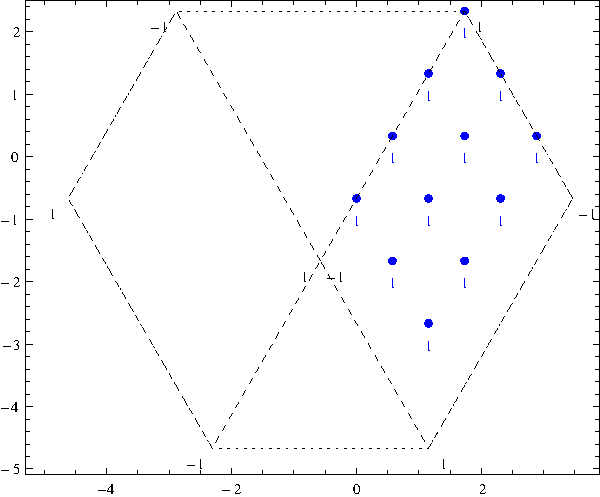
\includegraphics[width=80mm]{a2-a1}
  }
  \caption{Weyl group orbit (dotted) producing singular element of $L^{[3,2]}_{A_{2}}$ and its decomposition into the sum of splint images of singular elements of modules  $L^{[3,2]}_{A_{1}\oplus A_{1}}$ (dashed). Weight multiplicities of $L^{[3,2]}_{A_{1}\oplus A_{1}}$-module coincide with branching coefficients for the reduction $L^{[3,2]}_{A_{2}\downarrow A_{1}\oplus u(1)}$.}

 \label{fig:a2_splint}
\end{figure}
\end{example}
\begin{example}
  For the Lie algebra $B_{2}= \bf{so}(5)$ branching of its irreducible module $L^{[3,2]}$ into  modules of a reductive subalgebra $A_{1}\oplus u(1)$ with the root system spanned by the first simple root $\alpha_1=e_1-e_2$ of $B_{2}$. Singular element of $\Psi^{[3,2]}_{B_{2}}$ is decomposed into the sum of splint images of singular elements of $A_{2}$-modules and branching coefficients coincide with weight multiplicities of $A_{2}$-module (see Fig. \ref{fig:b2_splint}).

  \begin{figure}[h!bt]
  \hspace*{-1.2cm}

   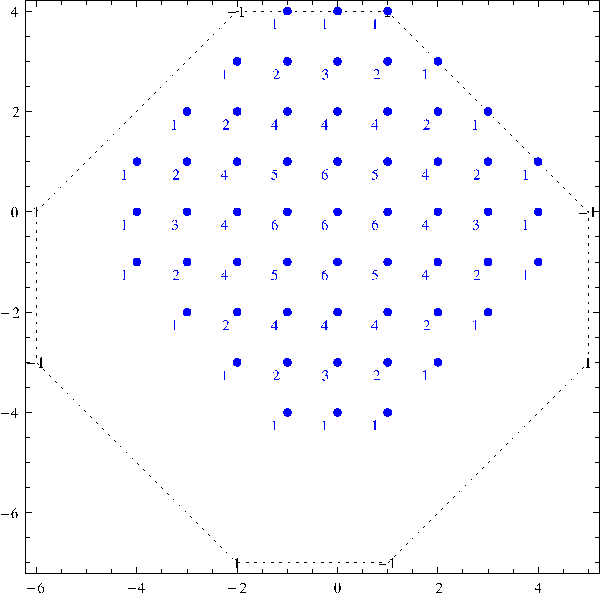
\includegraphics[width=65mm]{b2}
   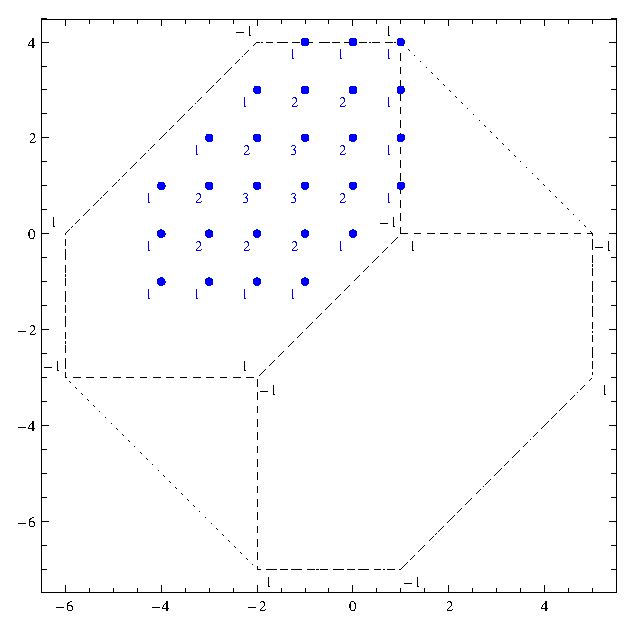
\includegraphics[width=65mm]{b2-a2-a1}
  \caption{Weights of the $B_{2}$-module $L^{[3,2]}$ are indicated by dots in the left picture (their multiplicities are also indicated). Contour of the singular element is shown by dotted line. The right picture presents the decomposition of  $\Psi_{B_{2}}(L^{[3,2]}_{B_{2}})$-singular element into the sum of splint images of singular elements $\Psi_{A_{2}}(L^{[3,2]})$ (dashed). Weight multiplicities of $L^{[3,2]}_{A_{2}}$-module coincide with branching coefficients for the reduction $L^{[3,2]}_{B_{2}\downarrow A_{1}\oplus u(1)}$.}

 \label{fig:b2_splint}
\end{figure}
\end{example}

\vspace{10mm}
\begin{example}
   Lie algebra $G_{2}$ has a regular subalgebra $A_{2}$ with root system $\Delta_{\af}=\Delta_{A_{2}}$ containing the $G_{2}$ long roots. Consider branching of an irreducible module $L_{G_{2}}^{(3,2)}$ into the $A_{2}$-modules. Singular element $\Psi_{G_{2}}(L^{[3,2]})$ is decomposed into the sum of splint images of singular elements $\Psi_{A_{2}}(L^{[3,2]})$ and the corresponding branching coefficients coincide with weight multiplicities of $L^{[3,2]}_{A_{2}}$-module (see Fig. \ref{fig:g2_splint}).


  \begin{figure}[h!bt]
  \noindent\centering{
   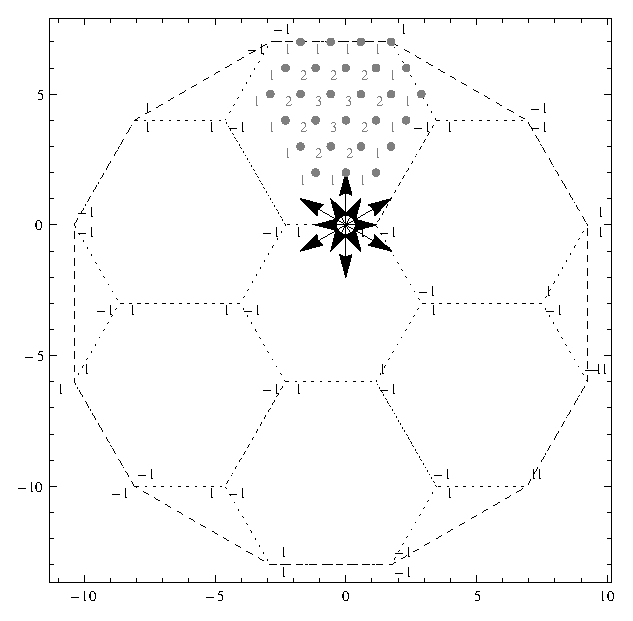
\includegraphics[width=120mm]{g2}
  }

  \caption{Weyl group orbit (dotted) for the singular element $\Psi_{G_{2}}(L^{[3,2]})$ and its decomposition into the sum of splint images of singular elements of $A_{2}$-modules (dashed). Weight multiplicities of $L^{[3,2]}_{A_{2}}$-module coincide with branching coefficients for the reduction $L^{[3,2]}_{G_{2}\downarrow A_{2}}$.}


 \label{fig:g2_splint}
\end{figure}

\end{example}

\section{Conclusions}

\label{sec:conclusions}It is explicitly demonstrated that splint
presents a very effective tool to find branching coefficients. In
particular injective splints provide a possibility to reduce
branching rules calculations for highest weight modules to a
determination of weight multiplicities for a module with the same
Dynkin labels referred to the Lie algebra $\mathfrak{s}$. This algebra
$\mathfrak{s}$ must not be a subalgebra in the initial $\gf$ , it
has the same rank $r_{\mathfrak{s}}=r$\ , but obviously less
"complicated" than $\gf$ -- only a subset of the initial root system is involved in the second stem $\Delta_{\mathfrak{s}}$.

It is significant that for the injections $D_{r}\hookrightarrow B_{r}$ , $%
D_{r}\hookrightarrow C_{r}$ and $A_{r-1}\oplus u\left( 1\right) \hookrightarrow A_{r}$ splint technique shows
transparently Gelfand-Tzeytlin rules for branching:  the reduction is
multiplicity free (all nonzero
branching coefficients are equal to 1). Here it is an immediate consequence of the
structure of the second stem being a direct sum of $A_{1}$
algebras and the fact that the corresponding module
$L_{\sfr}^{\mu }$ is irreducible.


%%%%%%%%%%%%%%%%%%%%%%%%%%%%%%%%%%%%%%%%%%%%%%%%%%%%%%%%%%%%%


%%%%%%%%%%%%%%%%%%%%%%%%%%%%%%%%%%%%%%%%%%%%%%%%%%%%%%%%%%%%%
\section*{Appendix}

%%%%%%%%%%%%%%%%%%%%%%%%%%%%%%%%%%%%%%%%%%%%%%%%%%%%%%%%%%%%%

Let us demonstrate that for injective splints of classical Lie
algebras the following property is valid:
\begin{Prop}
Let $\Delta \approx (\Delta _{\af},\Delta _{\sfr})$ be an
injective
splint with the decomposition of simple roots $S=S_{\frak{c}}\cup S_{\frak{d}%
}$ with $S_{\frak{c}}=S\cap S_{\af}$ and $S_{\frak{d}}=S\cap S_{\sfr%
}$.
\end{Prop}
Thus for any simple root $\beta \in S_{\sfr}$ there exists the
pair of
roots ( $\alpha $ ,$\beta ^{\prime }$) with $\alpha \in $ $S_{\frak{c}%
},\beta ^{\prime }\in S_{\sfr}$ such that $\alpha =\beta
-\beta ^{\prime }$

\begin{itemize}
\item
Type 1. $\Delta _{G_{2}}\approx (\Delta _{A_{2}},\Delta
_{A_{2}}).$

 \begin{figure}[h!bt]
  \noindent\centering{
   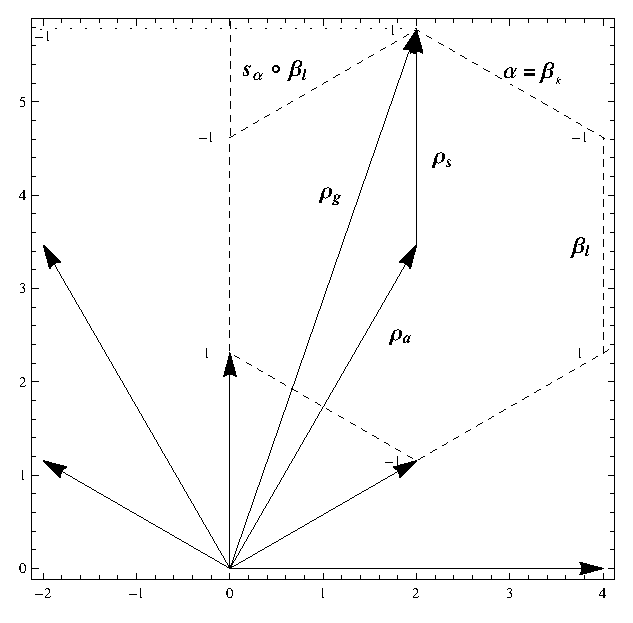
\includegraphics[width=100mm]{g2-roots}
  }
  \caption{Positive roots of $G_{2}$ and formation of singular element $\Phi^{(0)}_{\mathfrak{s}}$ in the main Weyl chamber of $\af=A_{2}$.}
\end{figure}
Here both stems are metric and the corresponding root systems are
equivalent. In Figure 4 a part of the singular element $\Phi
_{G_{2}}^{\left( 0\right) }$ is presented. The boundaries of $\bar{C_{\frak{a%
}}}$ are the dashed lines starting at the center of the singular
element. It
contains the edge $\lambda _{2}=-\alpha _{2}=-\beta _{2}$ and the roots $%
-\beta _{1}=-s_{\alpha _{2}}\circ \beta _{3}$ and $ -\beta _{3}$
($\beta _{3}$ is indicated as $\beta _{l}$). For the root $\beta
_{1}$ the necessary pair
is  $(\alpha _{1}, \beta _{2})$: $\alpha _{1}=\beta _{1}-\beta _{2}$. The $%
\lambda _{2,3}^{\sfr}=\beta _{3}$ edge is equal to $\lambda _{1}^{\frak{s%
}}=\beta _{1}=s_{\alpha _{2}}\circ \beta _{3}$ and $m_{1}$ index
is aquired by the $\sfr$-module that also inherit the second
index $m_{2}$. In this particular
case they are $m_{1}=m_{2}=0$. The general case with the initial module $%
L^{\mu }$ and $\mu =m_{1}\omega _{1}+m_{2}\omega _{2}$ can be
treated in the same way: one finds an edge $\lambda _{2}=-\left(
m_{2}+1\right) \beta _{2}$ and put $\lambda
_{1}^{\sfr}=-\left( m_{1}+1\right) \beta _{1}$, its end
belongs to the boundary $\bar{C_{\af}}$. The reflection
$s_{\beta
_{2}} $ sends $\beta _{1}$ to $\beta _{3}$ and the corresponding edge 
$\lambda _{2,3}^{\sfr}=-\left( m_{1}+1\right) \beta _{3}$ has
the length $\left( m_{1}+1\right) $. Now consider $\lambda _{1}^{\sfr}$ (or
$\lambda _{2,3}^{\sfr} $) and $\lambda _{1,3}^{\sfr}$ (or
$\lambda _{2,3,1}^{\sfr}$) edges to find that they belong to
the boundary $\bar{C_{\af}}$ and the Weyl symmetry predicts
that $\lambda _{1,3}^{\sfr}=-\left( m_{2}+1\right)
\beta _{3}$ ($\lambda _{2,3,1}^{\sfr}=-\left( m_{2}+1\right) \beta _{1}$%
) . Finally the edge $\lambda _{1,3,2}^{\sfr}=-\left(
m_{1}+1\right) \beta _{2}$ closes the polytope. Its vertices
correspond to weights of the singular
element $\Phi _{\sfr}^{\left( \widetilde{\mu }\right) }=\sum_{w\in W_{%
\sfr}}\varepsilon \left( w\right) e^{w\circ \left(
\widetilde{\mu }+\rho
_{\sfr}\right) }$ of the module $L_{\sfr}^{\left( \widetilde{\mu }%
\right) }$ with $\widetilde{\mu }=m_{1}\widetilde{\omega }_{1}+m_{2}%
\widetilde{\omega }_{2}$. Notice that in this case the sign
factors can be obtained directly in the initial weight system as
far as the stem is metric.
\item
Type 1. $\Delta _{F_{4}}\approx (\Delta _{D_{4}},\Delta
_{D_{4}}).$

Both stems are metric here and the corresponding root systems are
equivalent. The system $\Delta _{D_{4}}$ of the subalgebra
$\frak{a=}D_{4}$ is formed by the set $\left\{ \pm e_{i}\pm
e_{j}\right\} _{|i,j=1,\ldots 4,\; i\neq j}.$ The simple roots
$S_{\frak{c}}$ are $\left\{ e_{2}-e_{3},e_{3}-e_{4}\right\} $ and
$S_{\frak{d}}=\left\{ e_{4},\frac{1}{2}\left(
e_{1}-e_{2}-e_{3}-e_{4}\right) \right\} $.
For a module $L^{\mu }$ with $\mu =\sum m_{k}\omega _{k}$ consider the edge $%
\lambda _{3}=-\left( m_{3}+1\right) e_{4}=-\left( m_{3}+1\right)
\beta _{3}$.
 Compose an edge $\lambda _{2}^{\sfr}=-\left( \widetilde{m}%
_{2}+1\right) \beta _{2}$. The necessary pair of roots is $\left(
\alpha
_{2}=e_{3}-e_{4},\beta _{3}\right) $. The intersection of $\lambda _{2}^{%
\sfr}$ with the $\alpha _{2}$-boundary of
$\bar{C_{\af}}$ fixes
its length to be $\lambda _{2}^{\sfr}=-\left( m_{2}+1\right) \beta _{2}$%
\ and the length of the edge $\lambda _{3,2}^{\sfr}$ is equal
to that of
$\lambda _{2}^{\sfr}$. Next consider the edge $\lambda _{2}^{\sfr%
}=-\left( m_{2}+1\right) \beta _{2}$ and the pair $\left( \alpha
_{1}=e_{2}-e_{3},\beta _{1}=e_{2}\right) $. The length of  
$\lambda _{1}^{\sfr}$ becomes equal to $\lambda
_{1}^{\sfr}=-\left( m_{1}+1\right) \beta _{1}$. Proceed further till the closure of the polytope. 
The edges looking along the roots of the $\alpha_4$-type, $\alpha _{4}=\beta
_{4}=$ $\frac{1}{2}\left( e_{1}-e_{2}-e_{3}-e_{4}\right) $, are
treated similarly and finally the singular element $\Phi
_{\sfr}^{\left( \widetilde{\mu }\right) }=\sum_{w\in
W_{\sfr}}\varepsilon \left( w\right) e^{w\circ \left(
\widetilde{\mu }+\rho _{\sfr}\right) }$ for the module
$L_{\sfr}^{\left( \widetilde{\mu }\right) }$ with
$\widetilde{\mu }=\sum m_{k}\widetilde{\omega }_{k}$ is formed in
$\bar{C_{\af}}$.
\item
Type 2. $\Delta _{B_{r}}\approx (\Delta _{D_{r}},\Delta _{\oplus
^{r}A_{1}}). $

Both stems are metric. An injection is fixed by the stem $\Delta
_{D_{r}}$ simple roots $S_{\af}=\left\{
e_{1}-e_{2},e_{2}-e_{3},\ldots
,e_{r-1}-e_{r},e_{r-1}+e_{r}\right\} $. The second stem
corresponds to a
direct sum of algebras $A_{1}$ with the simple roots $S_{\sfr%
}=\left\{ e_{1},e_{2},\ldots ,e_{r-1},e_{r}\right\} $. Consider the edge $%
\lambda _{r}=-\left( m_{r}+1\right) \beta _{r}$ (here $\beta
_{r}=e_{r}$) and $\lambda _{r-1}=-\left(
\widetilde{m}_{r-1}+1\right) \beta _{r-1}$
attached to it (here $\beta _{r-1}=e_{r-1}$). The corresponding pair is $%
\left( \alpha _{r-1}=e_{r-1}-e_{r},\beta _{r-1}=e_{r-1}\right) $.
 The intersection condition fixes the second edge to be $\lambda
_{r-1}=-\left( m_{r-1}+1\right) \beta _{r-1}$ , it is orthogonal
to $\beta _{r}$ so the opposite edge has the same length. The
Dynkin index $m_{r-1}$ now refers
also to the\ simple root $\beta _{r-1}$. Next consider the obtained edge $%
\lambda _{r-1}=-\left( m_{r-1}+1\right) \beta _{r-1}$ and $\lambda
_{r-2}=-\left( \widetilde{m}_{r-2}+1\right) \beta _{r-2}$ to
fix the index $\widetilde{m}_{r-2}=m_{r-2}$ and the edge
$\lambda _{r-2}=-\left( m_{r-2}+1\right) \beta _{r-2}$ and so on
till all the pairs of edges are properly fixed. Finally in
$\bar{C}_{D_{r}}$ the element $\Phi _{\oplus ^{r}A_{1}}^{\left(
\widetilde{\mu }\right) }=\sum_{w\in W_{\oplus
^{r}A_{1}}}\varepsilon \left( w\right) e^{w\circ \left( \widetilde{\mu }+%
\frac{1}{2}\sum e_{k}\right) }$ can be constructed for the module
$L_{\oplus ^{r}A_{1}}^{\left( \widetilde{\mu }\right) }$ with
$\widetilde{\mu }=\sum m_{k}\frac{1}{2}e_{k}$.

\item
Type 2. $\Delta _{C_{r}}\approx (\Delta _{D_{r}},\Delta _{\oplus
^{r}A_{1}}). $

The situation in this case is eqivalent to the previous one and
the additional edges are constructed similarly.
\item
Type 3 $\Delta _{A_{r}}\approx (\Delta _{A_{r-1}\oplus
u_{1}},\Delta _{\oplus ^{r}A_{1}}).$

Here only the first stem is metric and it fixes the injection with
simple roots $S_{\af}=\left\{ e_{1}-e_{2},e_{2}-e_{3},\ldots
,e_{r-1}-e_{r}\right\} $. The second stem corresponding to a direct sum of $%
r$ copies of $A_{1}$ has the simple roots $S_{\sfr}=\left\{
e_{1}-e_{r+1},e_{2}-e_{r+1},\ldots ,e_{r}-e_{r+1}\right\} $.
Consider the edge $\lambda _{r}=-\left( m_{r}+1\right) \beta _{r}$
with $\beta
_{r}=e_{r}-e_{r+1}$ and $\lambda _{r-1}=-\left( \widetilde{m}%
_{r-1}+1\right) \beta _{r-1}$ \ with $\beta
_{r-1}=e_{r-1}-e_{r+1}$ attached to it. Then the corresponding
pair is $\left( \alpha _{r-1}=e_{r-1}-e_{r},\beta
_{r-1}=e_{r-1}-e_{r+1}\right)$. The intersection with the
boundary of $\bar{C}_{A_{r-1}}$ orthogonal to $\alpha _{r-1}$
fixes the second edge to be $\lambda _{r-1}=-\left(
m_{r-1}+1\right) \beta _{r-1}$. The Dynkin index $m_{r-1}$ is to
be used for the fundamental weight  $\omega _{r-1}.$ The\
reflection $s_{\beta _{r}}$ sends $\lambda _{r-1}=-\left(
m_{r-1}+1\right) \beta _{r-1}$ to $\lambda _{r,r-1}=-\left(
m_{r-1}+1\right) \beta _{r-1}.$ Next consider the obtained edge
$\lambda _{r-1}=-\left( m_{r-1}+1\right) \beta _{r-1}$ and
$\lambda _{r-2}=-\left( \widetilde{m}_{r-2}+1\right) \beta _{r-2}$
with $\beta _{r-2}=e_{r-2}-e_{r+1} $ to obtain the index
$\widetilde{m}_{r-2}=m_{r-2}$ and the edge $\lambda _{r-2}=-\left(
m_{r-2}+1\right) \beta _{r-2}$ and so on till all the pairs of
edges are properly fixed. Finally in $\bar{C}_{D_{r}}$ the element
$\Phi _{\oplus ^{r}A_{1}}^{\left( \widetilde{\mu }\right)
}=\sum_{w\in W_{\oplus
^{r}A_{1}}}\varepsilon \left( w\right) e^{w\circ \left( \widetilde{\mu }+%
\widetilde{\rho }\right) }$ can be constructed for the module
$L_{\oplus ^{r}A_{1}}^{\left( \widetilde{\mu }\right) }$ with
$\widetilde{\mu }=\sum m_{k}\beta _{k}.$ The simplest case
$\Delta _{A_{2}}\approx (\Delta _{A_{1}\oplus u_{1}},\Delta
_{A_{1}\oplus A_{1}})$ is presented in Example 4.1 and Figure 1.
\item
Type 3 $\Delta _{B_{2}}\approx (\Delta _{A_{1}},\Delta _{A_{2}}).$

This splint is illustrated in Example 4.1 and Figure 1, 
$S_{A\_1}=\left\{ e_{1}-e_{2}\right\} $, $S_{A\_2}=\left\{
e_{1},e_{2}\right\} $. The edge $\lambda _{\alpha _{2}}=\lambda
_{\beta _{2}}=-\left( m_{2}+1\right) \beta _{2}$ is followed by
$\lambda _{\beta _{1}}=-\left( \widetilde{m}_{1}+1\right) \beta
_{1}$. Consider the pair $\left( \alpha
_{1}=e_{1}-e_{2},\beta _{1}=e_{1}\right)$. The end of the edge
$\lambda _{\beta _{1}}$ must indicate a weight
invariant under the reflexion $s_{\alpha _{1}}$.  Its length is thus fixed: 
$\lambda _{\beta _{1}}=-\left( m_{1}+1\right) \beta _{1}$. In the
coimage of
the second stem, that is in the root system $\Delta_{A_{2}}$, the reflection 
$s_{\beta _{2}}$ sends $\lambda _{\beta _{1}}=-\left(
m_{1}+1\right) \beta
_{1}$ to $\lambda _{2,3}$, thus the latter edge has the same length in $%
\beta _{3}=e_{1}+e_{3}$, we have $\lambda _{2,3}=-\left(
m_{1}+1\right)
\beta _{3}$ with $\beta _{3}=e_{1}+e_{3}$. The irreducible $\sfr$%
-module has the highest weight $\widetilde{\mu }=m_{1}\widetilde{\omega }%
_{1}+m_{2}\widetilde{\omega }_{2}$. In Figure 1 we see the
details of these relations in a particular case where
$L_{B_{2}}^{\left[ 3,2\right] }$ is reduced to a subalgebra
$A_{1}\oplus u\left( 1\right) $ and the
corresponding highest weights (with their multiplicities) form the diagram $%
\mathcal{N}_{A_2}^{\left[ 3,2\right] }$ .
\end{itemize}

%%%%%%%%%%%%%%%%%%%%%%%%%%%%%%%%%%%%%%%%%%%%%%%%%%%%%%%%%%%%%
%%%%%%%%%%%%%%%%%%%%%%%%%%%%%%%%%%%%%%%%%%%%%%%%%%%%%%%%%%%%%


%%
%% End of file
%%% Local Variables: 
%%% mode: latex
%%% TeX-master: "thesis"
%%% End: 
